\subsubsection{Purpose}
The reserve car feature is a key service of \emph{PowerEnJoy}. Its main purpose is that of allowing users to choose a nearby car from the ones marked as available on the map, hence signaling their intention of reserving it for an hour. The service can be accessed from the home page of both the web and mobile applications, clicking on the corresponding icon on the toolbar.

The reservation screen shows the user only available cars, based on the information provided by the server. The user can either search for an available car using the mobile application or the web application, indicating an address around which he wishes to search for a vehicle. If the user is logged in through the mobile application, he/she can also choose to use his/her GPS position - as provided by the mobile device - instead of a specific address.

Only one car should be rented at a time, so the system will prevent the user from trying to reserve several cars simultaneously.

\subsubsection{Scenario 1}
Alice is logged in to the \emph{PowerEnJoy} service with her laptop, because she wants to find a car to go meet a friend downtown. To do so, she clicks on the reservation icon and opens the city map. She inputs her address, to indicate that she wants a car not far from her house. The system proceeds to mark the vehicles within the desired location. Alice finds a car that she thinks is reasonably close and clicks on it. The system prompts her asking: \emph{"Do you really want to reserve this car?"}. She clicks on the \emph{"Confirm"} button, hence forwarding the request of the specific car to the system.

\subsubsection{Scenario 2}
Bob is in town and has just finished shopping. He wants to go back home, but does not want to catch a crowded subway train during the rush hour. For this reason he has logged in to the \emph{PowerEnJoy} application and taps on the reservation icon. The system opens a map that shows the GPS position - provided by Bob's smartphone - and several icons marking nearby available cars. He chooses a vehicle just around the corner and properly confirms his intention of reserving the car for some time; by doing so, his request is forwarded to the server. A few minutes later, he meets a friend that offers him a ride, and decides to accept. So, he logs in to his account again and opens the reservation function. He taps on the \emph{"Release Reservation"} button and the system processes his request by marking the car as available again.

\subsubsection{Scenario 3}
Carla is in need of a car after work, and decides to use a \emph{PowerEnJoy} one. She is looking at the reservation screen and decides to reserve a vehicle by selecting it. Since she is not sure that she will be able to reach the vehicle easily, she tries to reserve a second one after a few minutes. At that point, the system shows a visual recap of her current reservation. Carla tries to access the city map, but the system prevents her to do so, unless she cancels her current reservation. So she renounces to the second reservation and the system does not change anything about the active reservation status.

\subsubsection{Use-case}
A more detailed use-case diagram is provided in order to model the possibility of releasing an existing reservation. The detail of the use-case diagram is shown in Figure \ref{request_car_uc}.

The use-case for the standard procedure needed to request a car is analyzed in Table \ref{reserve_car_uc}.
The use-case for the procedure needed to release an existing reservation is analyzed in Table \ref{reserve_car_uc_alt}.

\subsubsection{Sequence diagram}
The diagram for the standard behavior of the system in case of a car reservation is shown in Figure \ref{reserve_car_sd}.

\subsubsection{Functional Requirements}
\begin{enumerate}
\item Only addresses within a distance of 2 km from the Safe Area boundaries must be considered valid;
\item If a user inputs a non-valid address, the system must notify him/her with an error message saying that he/she is too far from the Safe Area to locate a car nearby;
\item The system must only show available cars if they are within the Safe Area;
\item The system must provide the position of all nearby vehicles in a radius of 2 km precisely for every address that was considered valid;
\item The system must mark as available only cars that are not already reserved or out-of-service;
\item The system must check that only available vehicles can be rented;
\item The system must mark as reserved any rented vehicle;
\item An available car can be rented by only one registered user at a time;
\item If a user tries to reserve an car, but that car has been reserved by another user during the visualization of the available vehicles, the system must notify it with an error message;
\item The system must allow to reserve cars only users that do not have an active reservation, that is to say a reservation not older than an hour;
\item If a user has an active reservation, the system must show as first screen - upon the selection of the reservation function - the recap of said active reservation, including time of expiration and car location;
\item If a user has an active reservation, the system must allow him/her to renounce to it by clicking on the \emph{"Release reservation"} button and confirming his/her intentions;
\item The system must always notify the user of a successful reservation/recess from a reservation, immediately after the action is saved in memory by the server;
\item The system must allow the user to visualize the available cars without renting any, by canceling the current reservation procedure.
\end{enumerate}

\begin{figure}[H]
\begin{center}
		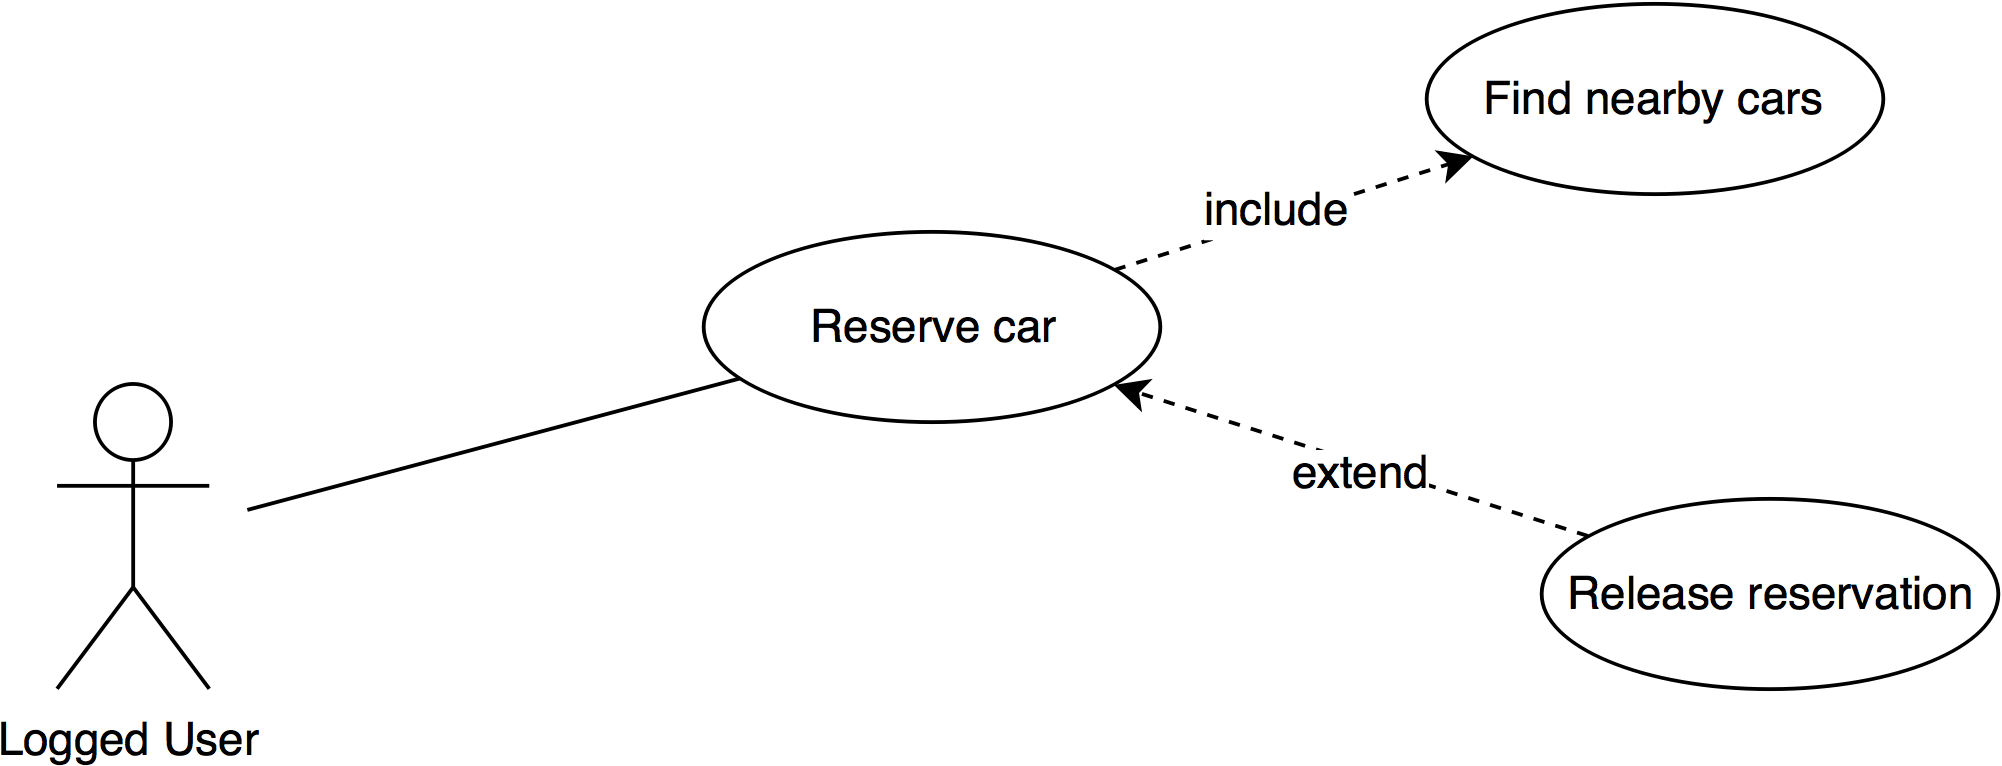
\includegraphics[width=\textwidth]{./specific_requirements/features/diagrams/request_car_uc.png}
		\caption{Extension of the use case diagram that includes the "Release reservation" feature}
		\label{request_car_uc}
\end{center}
\end{figure}

\begin{figure}[H]
\begin{center}
		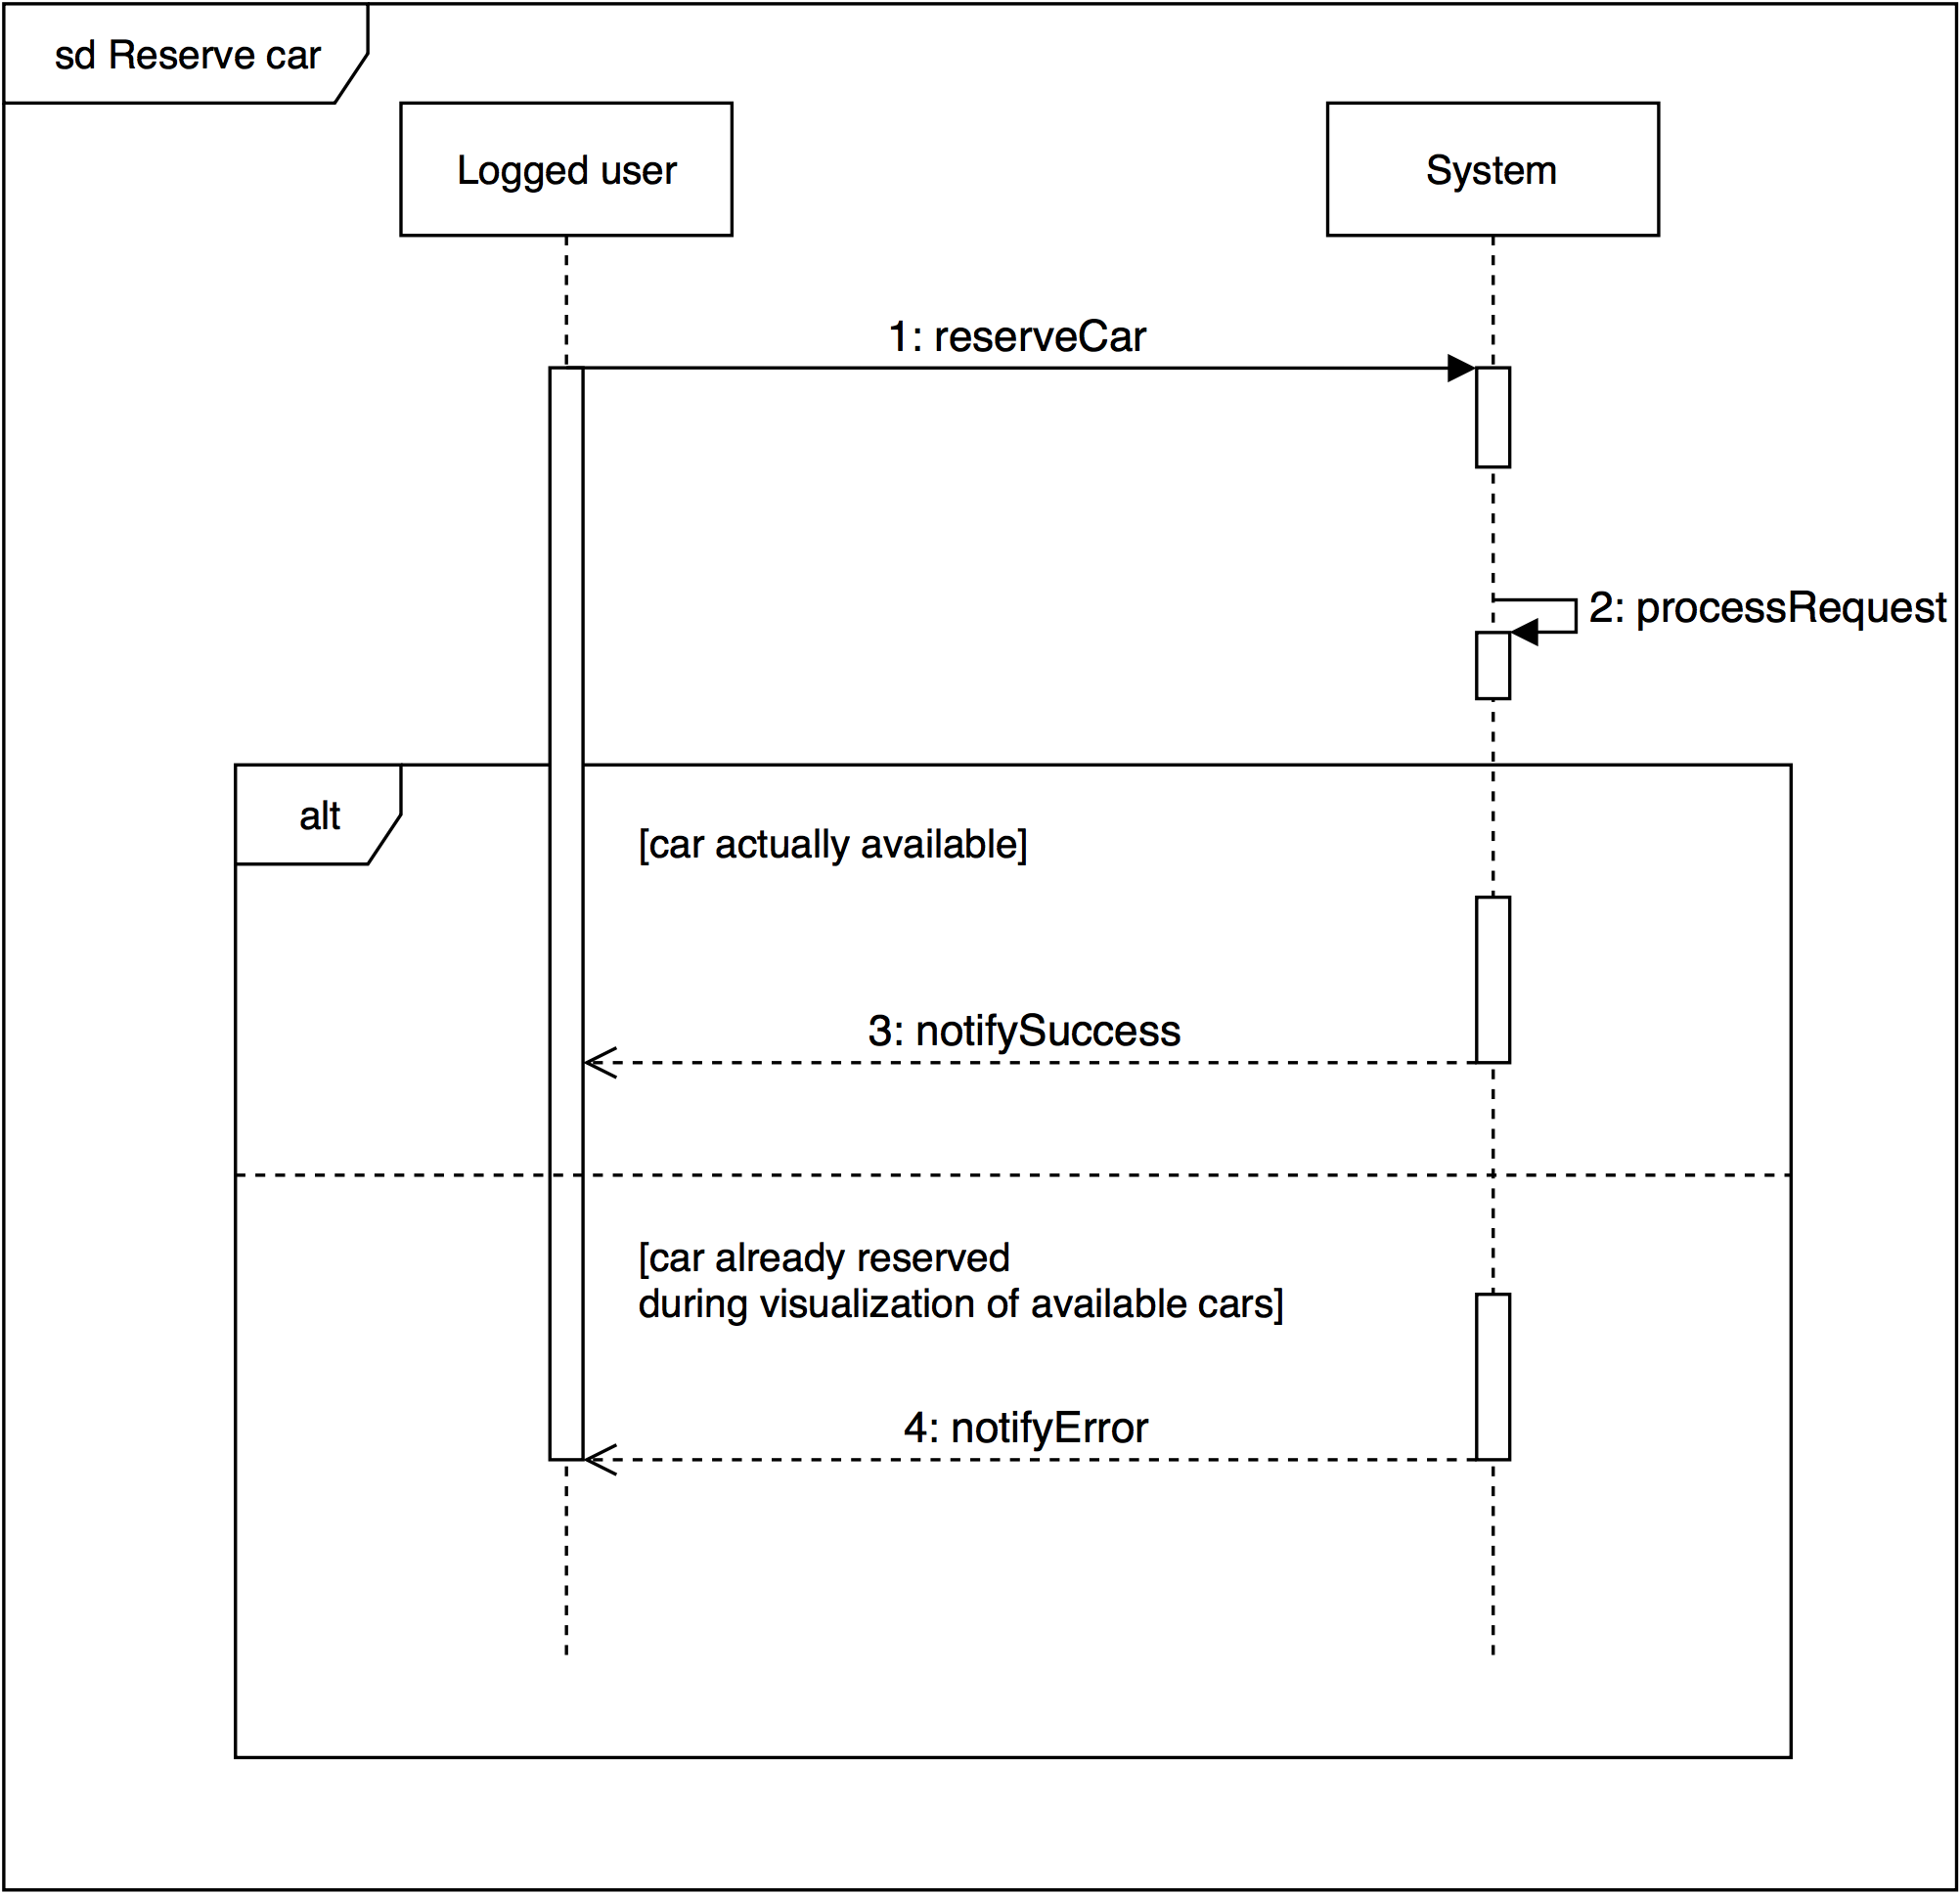
\includegraphics[width=\textwidth]{./specific_requirements/features/diagrams/reserve_car_sd.png}
		\caption{Sequence diagram that describes the event flow of a standard reservation request}
		\label{reserve_car_sd}
\end{center}
\end{figure}

\begin{table}[H]
\begin{center}
\begin{tabular}{p{0.3\textwidth} | p{0.7\textwidth}}
\hline
Actor & Logged user\\
\hline
Goal & Goal 3\\
\hline
Input Condition & The user is logged in and has no active reservations\\
\hline
Event Flow & 
\begin{enumerate}
\item In the main page for the \emph{PowerEnJoy} website or mobile application, the user clicks or taps on the \emph{"Reserve car"} button;
\item The user inputs the desired location: specific address or current GPS location;
\item The system loads a map of the Safe Area, marking every available vehicle near the desired location;
\item The user clicks or taps on the car he/she wants to rent;
\item The user clicks or taps on the \emph{"Confirm"} button when asked if he actually wants to rent the car;
\item The system saves the registration in its database and logs it;
\item The system confirms the reservation to the user, reminding him/her of the fact that the reservation will expire in an hour of time with a small fee if the car is not actually used.
\end{enumerate} \\
\hline
Output Condition & The system notifies the user that the reservation was successful and marks the chosen car as reserved.\\
\hline
Exception & If the user tries to reserve more than one car, the system notifies him/her that this action is forbidden.

If the user changes his/her mind and decides not to reserve a car, the event flow stops at the point in which the map was shown. No car will be reserved in this eventuality.\\
\hline
\end{tabular}
\end{center}
\caption{Reserve car use-case}
\label{reserve_car_uc}
\end{table}

\begin{table}[H]
\begin{center}
\begin{tabular}{p{0.3\textwidth} | p{0.7\textwidth}}
\hline
Actor & Logged User\\
\hline
Goal & Goal 3\\
\hline
Input Condition & The user is logged in and has an active reservation not older than an hour\\
\hline
Event Flow & 
\begin{enumerate}
\item In the main page for the \emph{PowerEnJoy} website or mobile application, the user clicks or taps on the \emph{"Reserve car"} button;
\item Since the user already reserved a car, he is shown the location and time of his current reservation;
\item The user clicks or taps on the \emph{"Release reservation"} button;
\item The system asks confirmation from the user;
\item The user confirms his/her choice of receding from his/her existing reservation;
\item The system modifies the state of the formerly reserved car marking it as available again and notifies the user of the fact that his/her reservation was successfully cancelled.
\end{enumerate} \\
\hline
Output Condition & The system notifies the user that the reservation was successfully cancelled and marks the chosen car as available again. The user can reserve another car, since he/she has no more active reservations\\
\hline
Exception & If the user changes his/her mind and wants to keep the current reservation, the event flow stops at the point in which the current reservation was shown. The reservation will be kept unchanged in this eventuality.\\
\hline
\end{tabular}
\end{center}
\caption{Reserve car use-case for the option of releasing a reservation}
\label{reserve_car_uc_alt}
\end{table}

\begin{figure}[H]
\begin{center}
		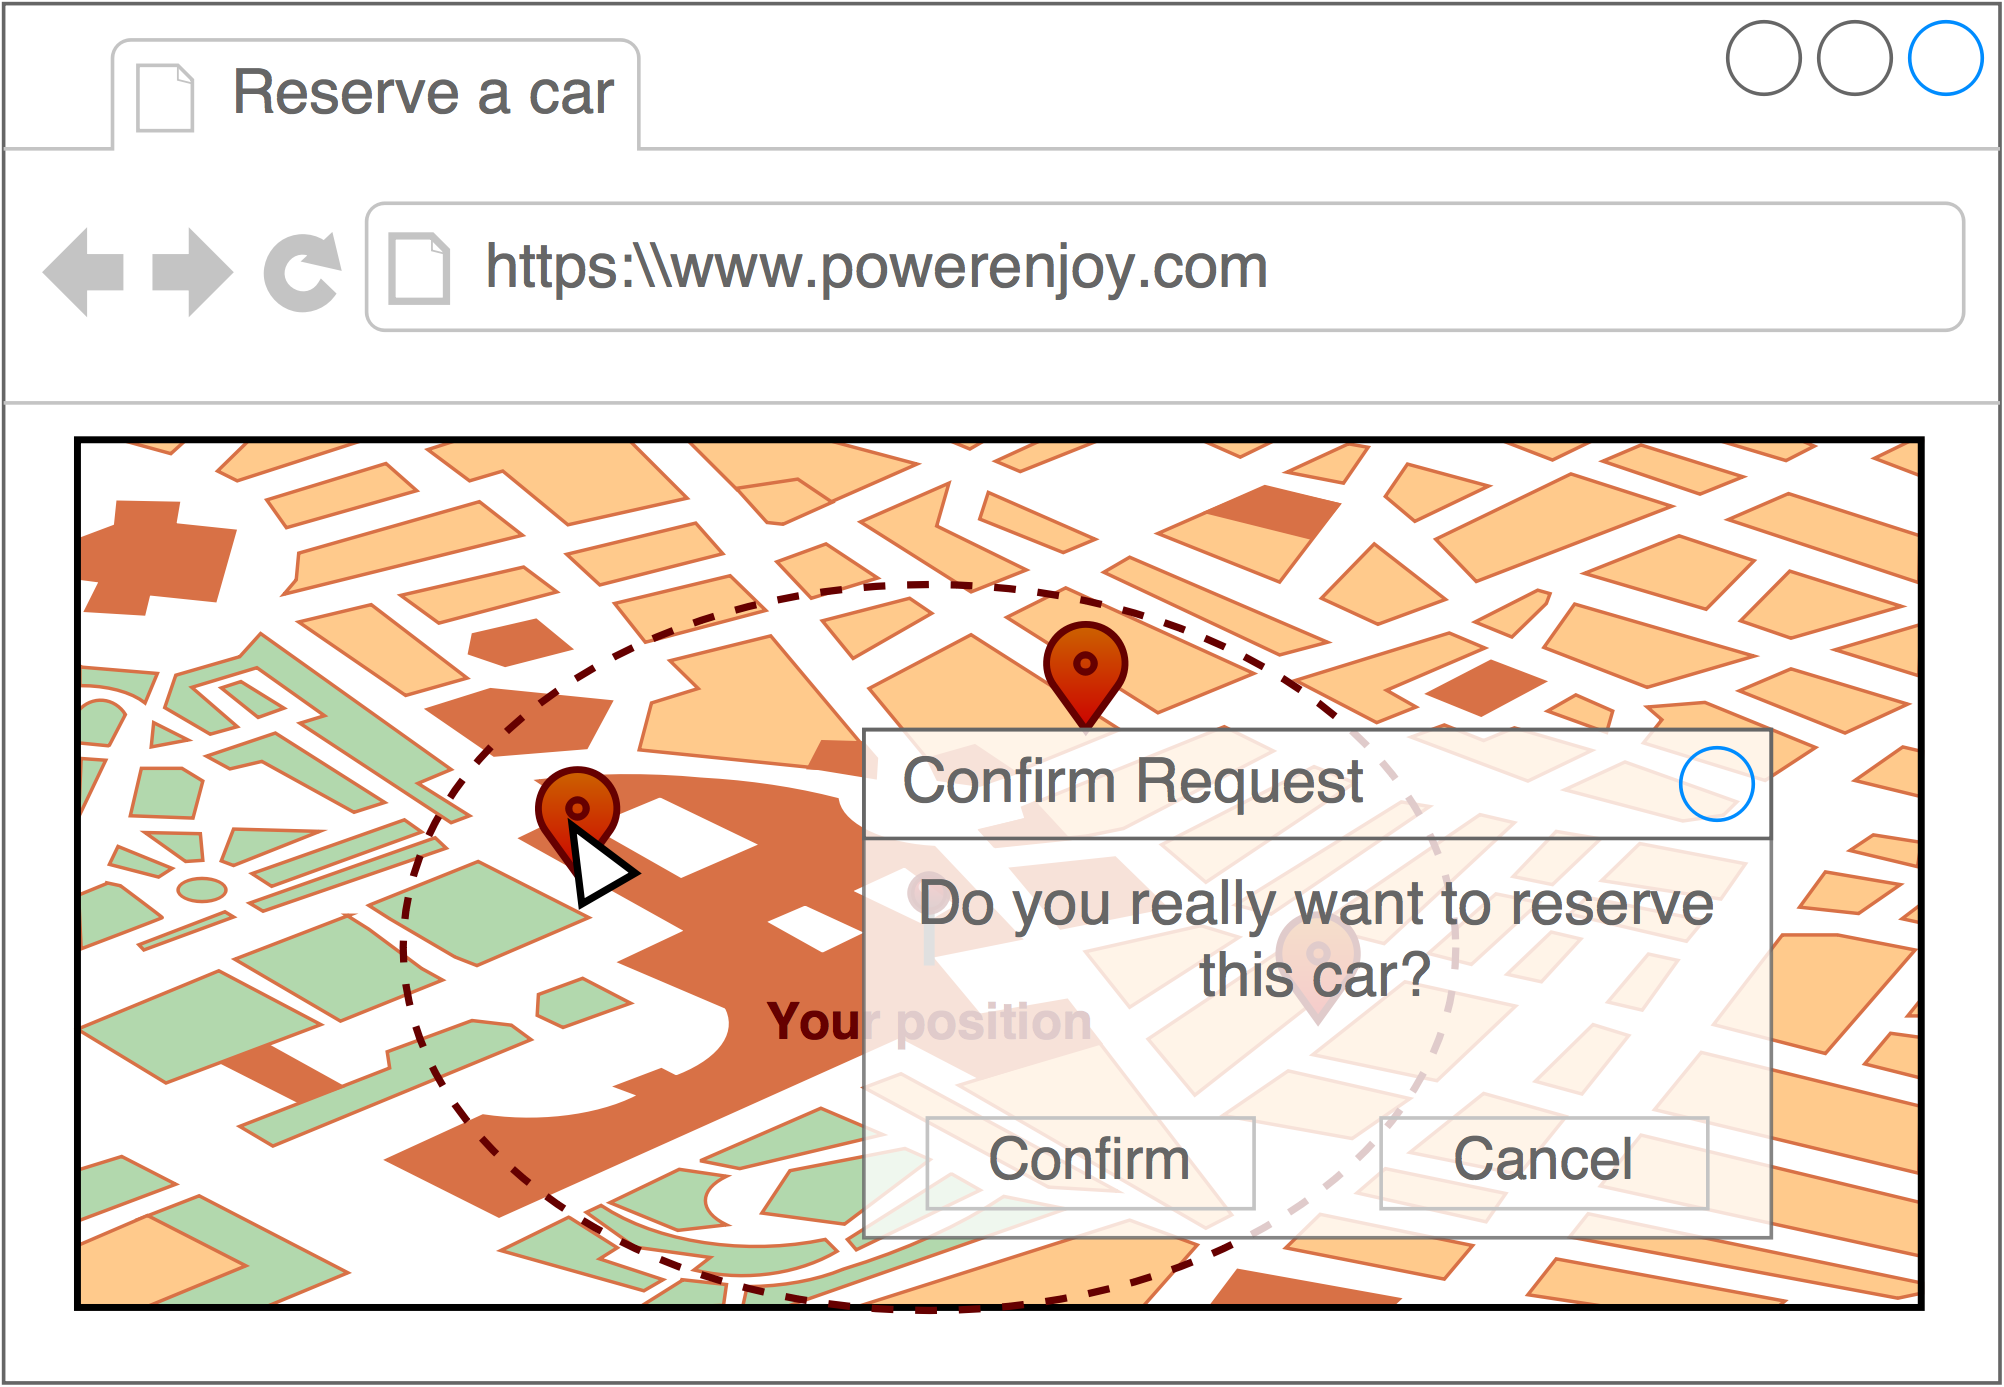
\includegraphics[width=0.9\textwidth]{./specific_requirements/features/diagrams/web_reserve_car.png}
		\caption{Mockup of the reservation web page}
		\label{web_reserve_car}
\end{center}
\end{figure}

\begin{figure}[H]
\begin{center}
		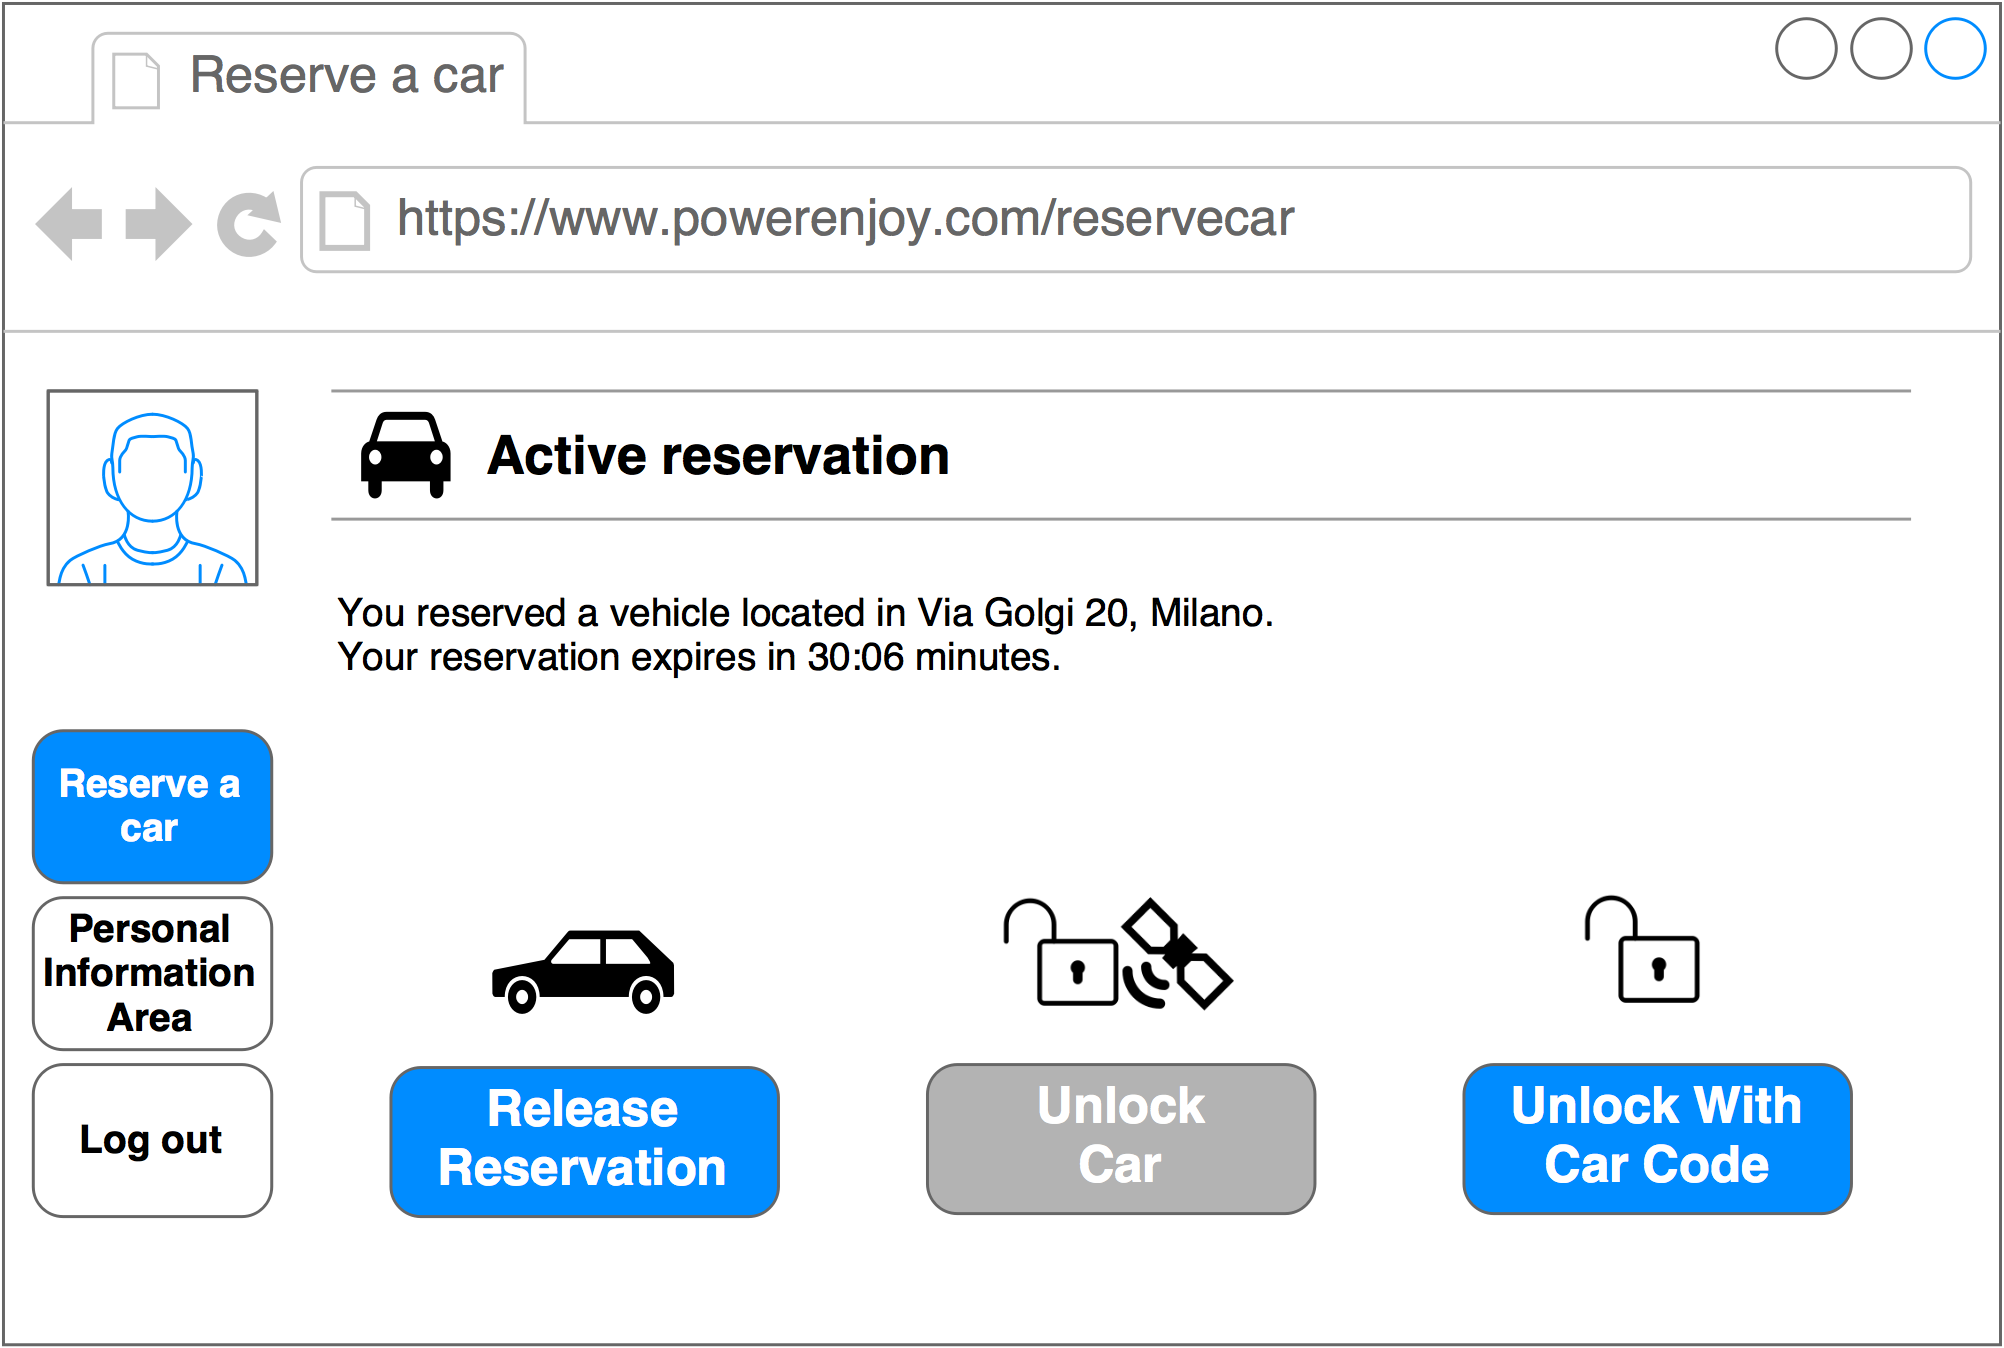
\includegraphics[width=0.9\textwidth]{./specific_requirements/features/diagrams/web_recap_reserv.png}
		\caption{Mockup of the reservation web page with a pending active reservation.}
		\label{web_recap_reserv}
\end{center}
\end{figure}